\chapter{Deployment, Testing and System Evaluation}
\section{System Testing}

Software testing \cite{katalon_software_testing} is the process of evaluating software to ensure it meets expected requirements. Testers run the software in controlled environments across various scenarios to identify any problems before release.

\paragraph{Why Testing Matters}

\begin{itemize}
    \item \textbf{Bug Detection}: Testing finds problems early, preventing cascading failures in interconnected systems.
    \item \textbf{Quality Assurance}: Testing ensures software remains stable, secure, and user-friendly while highlighting areas for improvement.
    \item \textbf{User Trust}: Reliable, well-tested products create positive user experiences and build customer confidence.
    \item \textbf{Risk Management}: In critical industries like healthcare and finance, testing prevents potentially harmful errors and protects against legal exposure.
\end{itemize}

\paragraph{Main Testing Categories}

Software testing falls into two primary categories:

\begin{itemize}
    \item \textbf{Functional Testing}: Verifies that features work correctly as specified
    \item \textbf{Non-functional Testing}: Examines qualities like performance, security, and usability
\end{itemize}

\paragraph{Common Testing Approaches}

The testing landscape includes many specialized methods:

\begin{itemize}
    \item \textbf{Unit Testing}: Examines individual components in isolation
    \item \textbf{Integration Testing}: Checks how components work together
    \item \textbf{End-to-End Testing}: Validates complete workflows
    \item \textbf{System Testing}: Evaluates the entire system's functionality
    \item \textbf{Exploratory Testing}: Involves freestyle investigation to discover unexpected issues
    \item \textbf{Visual Testing}: Confirms visual elements appear correctly
    \item \textbf{Regression Testing}: Ensures new code doesn't break existing features
    \item \textbf{UI Testing}: Checks user interface elements and interactions
    \item \textbf{Black-Box Testing}: Tests without knowledge of internal code
    \item \textbf{White-Box Testing}: Tests with full knowledge of code structure
    \item \textbf{Cross-Browser Testing}: Verifies compatibility across different browsers
    \item \textbf{Acceptance Testing}: Validates against real-world scenarios
    \item \textbf{Performance Testing}: Measures behavior under stress conditions
\end{itemize}
\subsection{API Testing}
For our backend application development, we implemented Postman \cite{postman_api_testing} as our solution for API storage, synchronization among team members, and manual testing procedures.
\begin{figure}[H]
    \centering
    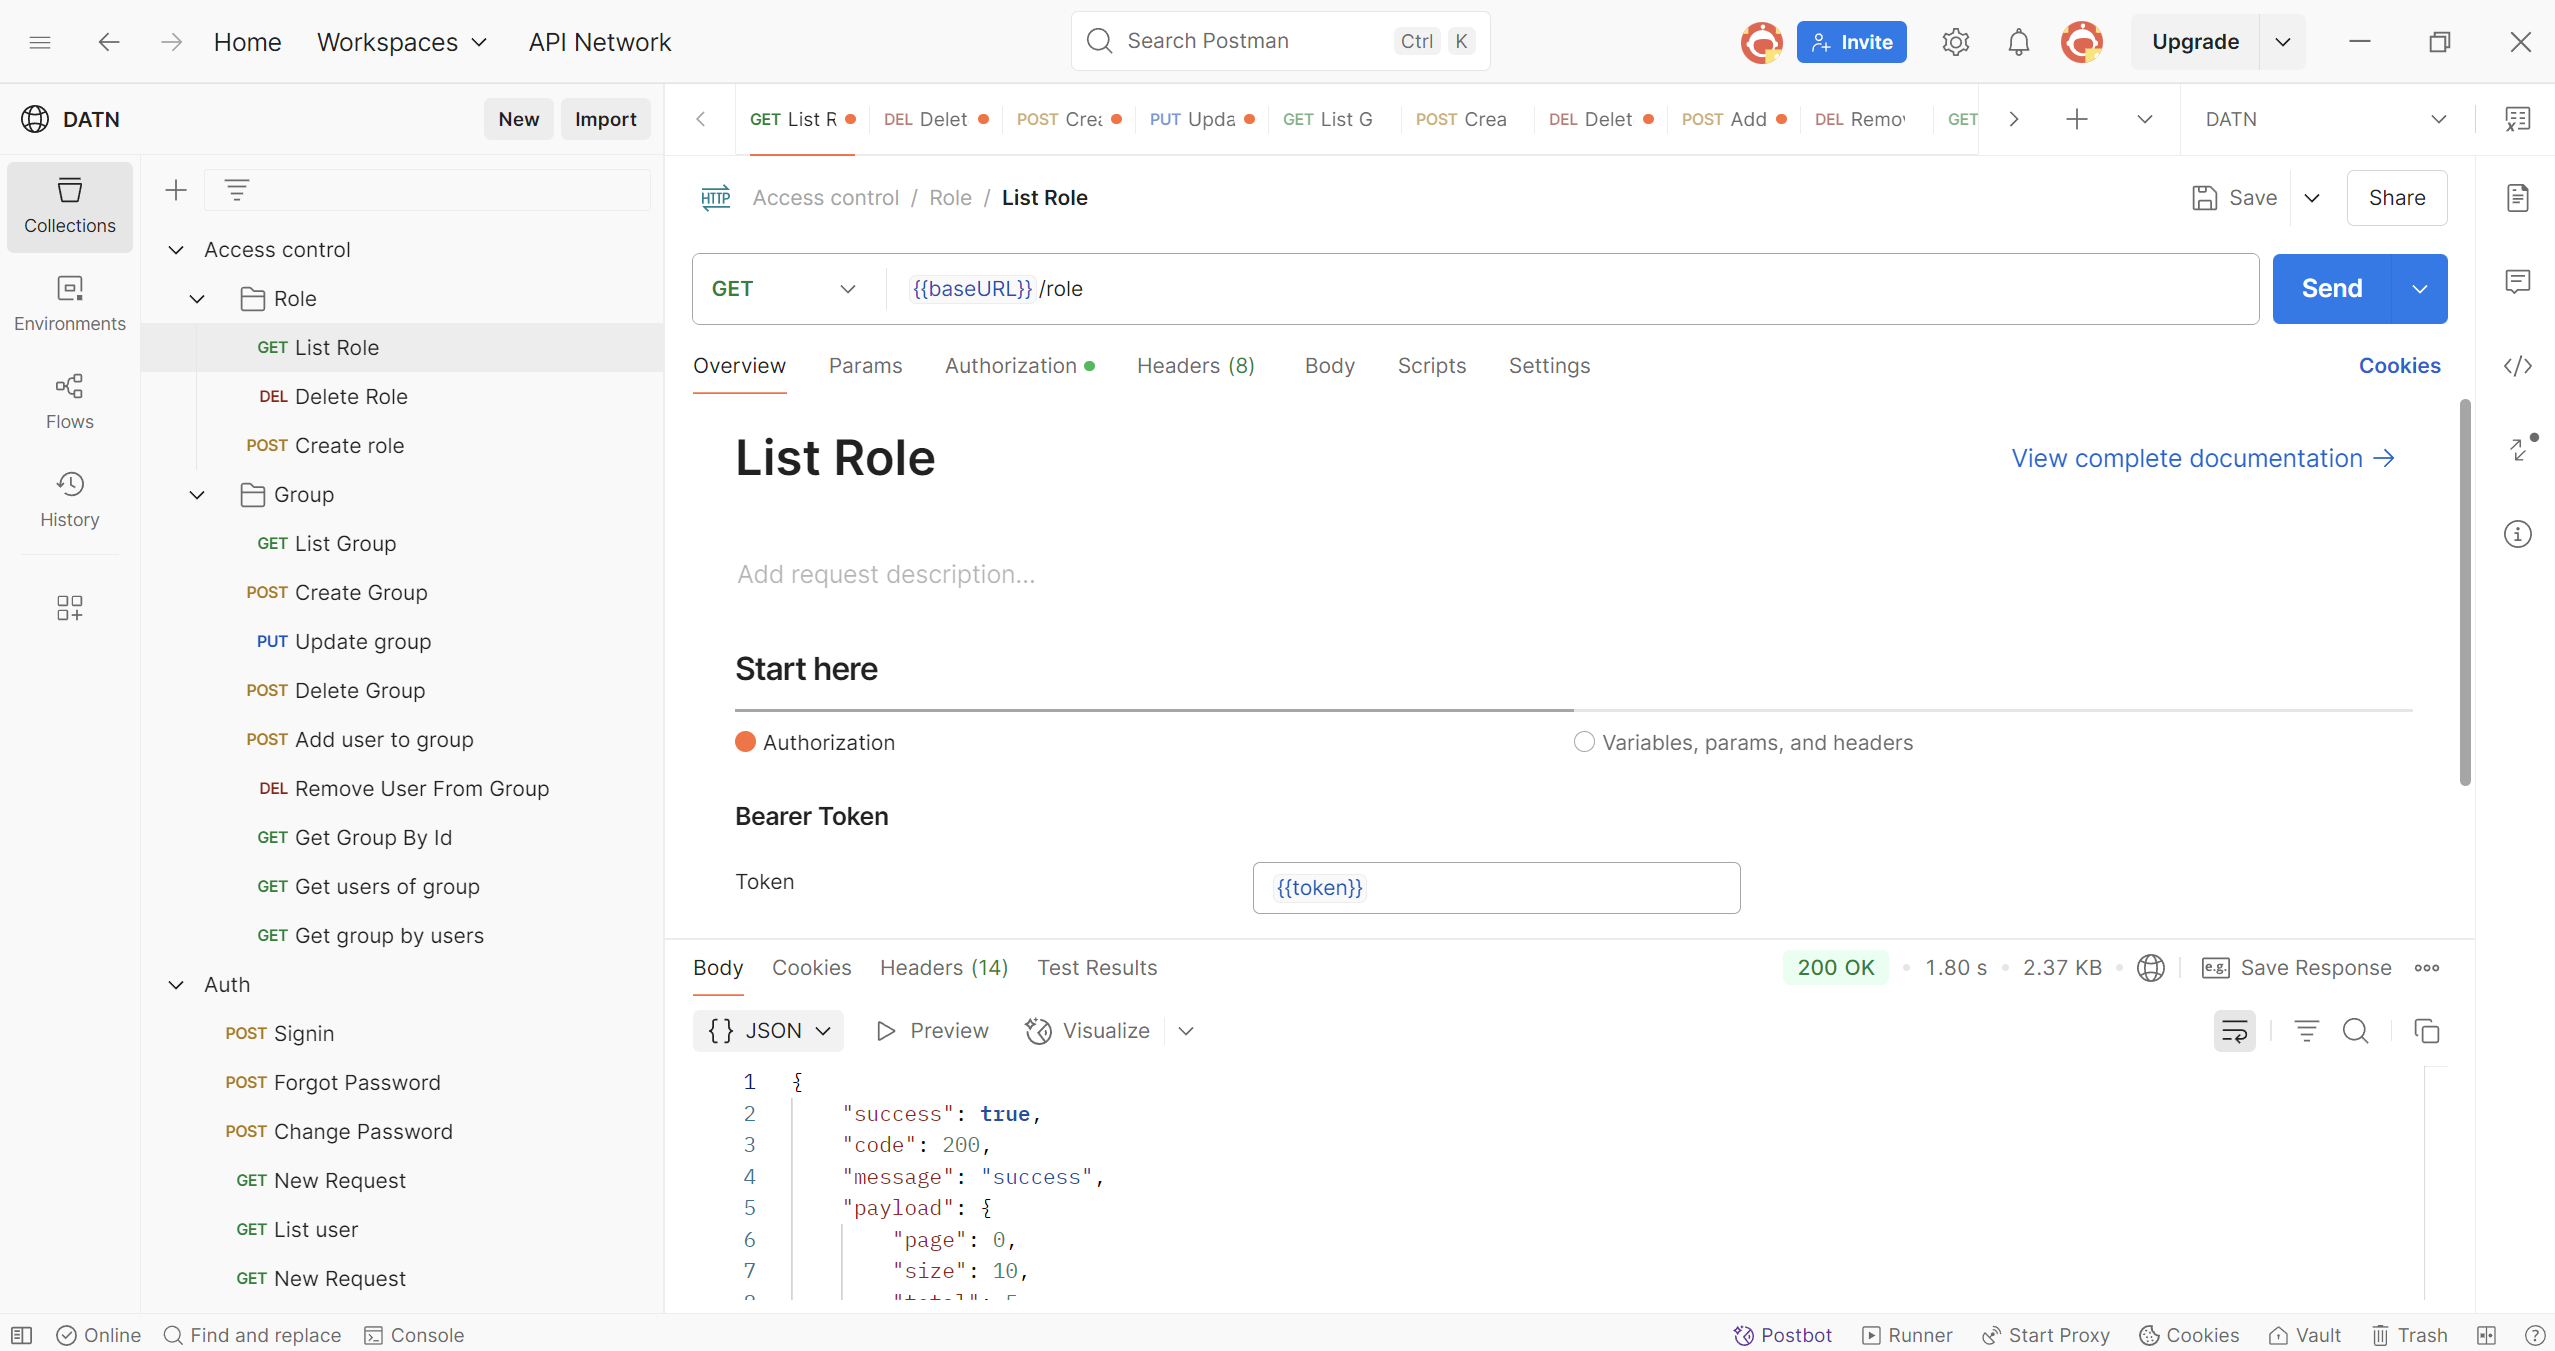
\includegraphics[width=15cm]{graphics/chapter6/postmain.png}
    \caption{API Testing with Postman}
    \label{fig:postman}
\end{figure}
\subsection{Web Interface Testing}

\section{Deployment}
\subsection{Frontend Deployment}
\subsection{Backend Deployment}

\section{System Evaluation}
Google PageSpeed Insights \cite{google_page_speed} is a suite of tools developed by Google designed to optimize web page performance. It primarily focuses on two key aspects: page loading speed and user experience. These components adhere to Google's web performance methodologies while automating the optimization process.

Google offers Lighthouse, an open-source automated tool aimed at improving website quality using the Google PageSpeed metrics. Users can apply this tool to any website, and it has the capability to access browser-stored data such as tokens. This Google Chrome Audit tool evaluates various aspects including performance, accessibility, SEO, and other parameters, providing corresponding scores.

To assess website performance using Lighthouse, users need to install the Lighthouse extension, open DevTools, select the Lighthouse tab, and choose ``Analyze page load." Lighthouse then runs a series of tests on the page and compiles the results into a comprehensive performance report. Based on these findings, users can make targeted improvements to enhance their website's overall performance.
\subsection{Evaluation results}
Using Lighthouse to evaluate the performance of our web application, we obtained the following results:
\begin{figure}[H]
  \centering
  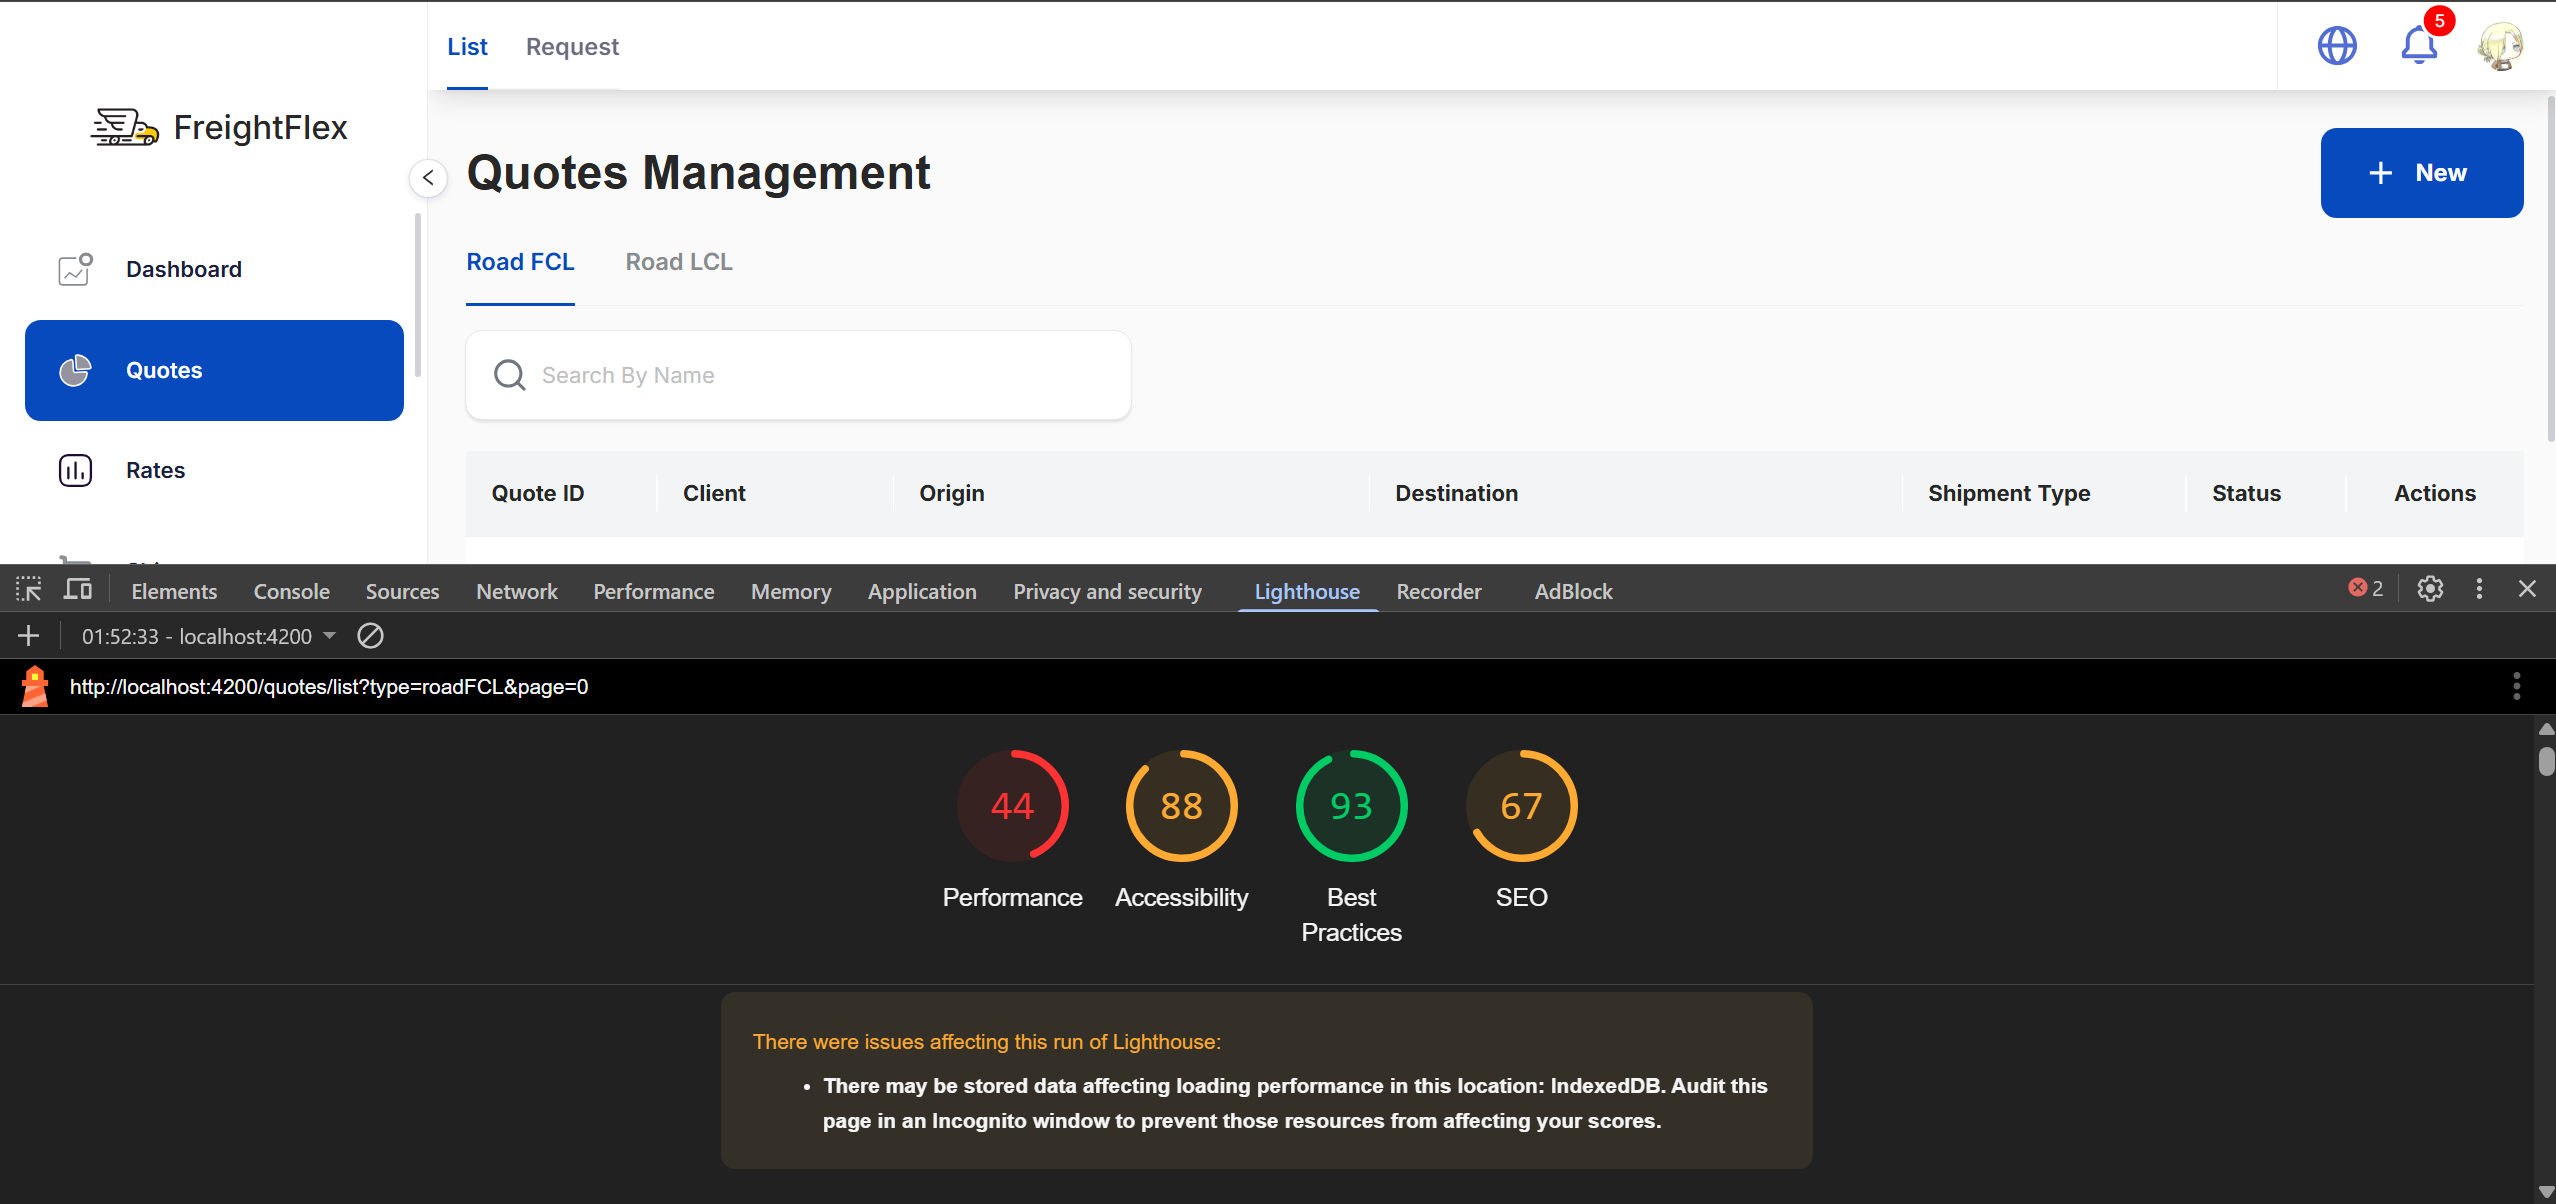
\includegraphics[width=15cm]{graphics/chapter6/quotes.png}
  \caption{Quotes page performance evaluation}
  \label{fig:quotes}
\end{figure}

\begin{figure}[H]
  \centering
  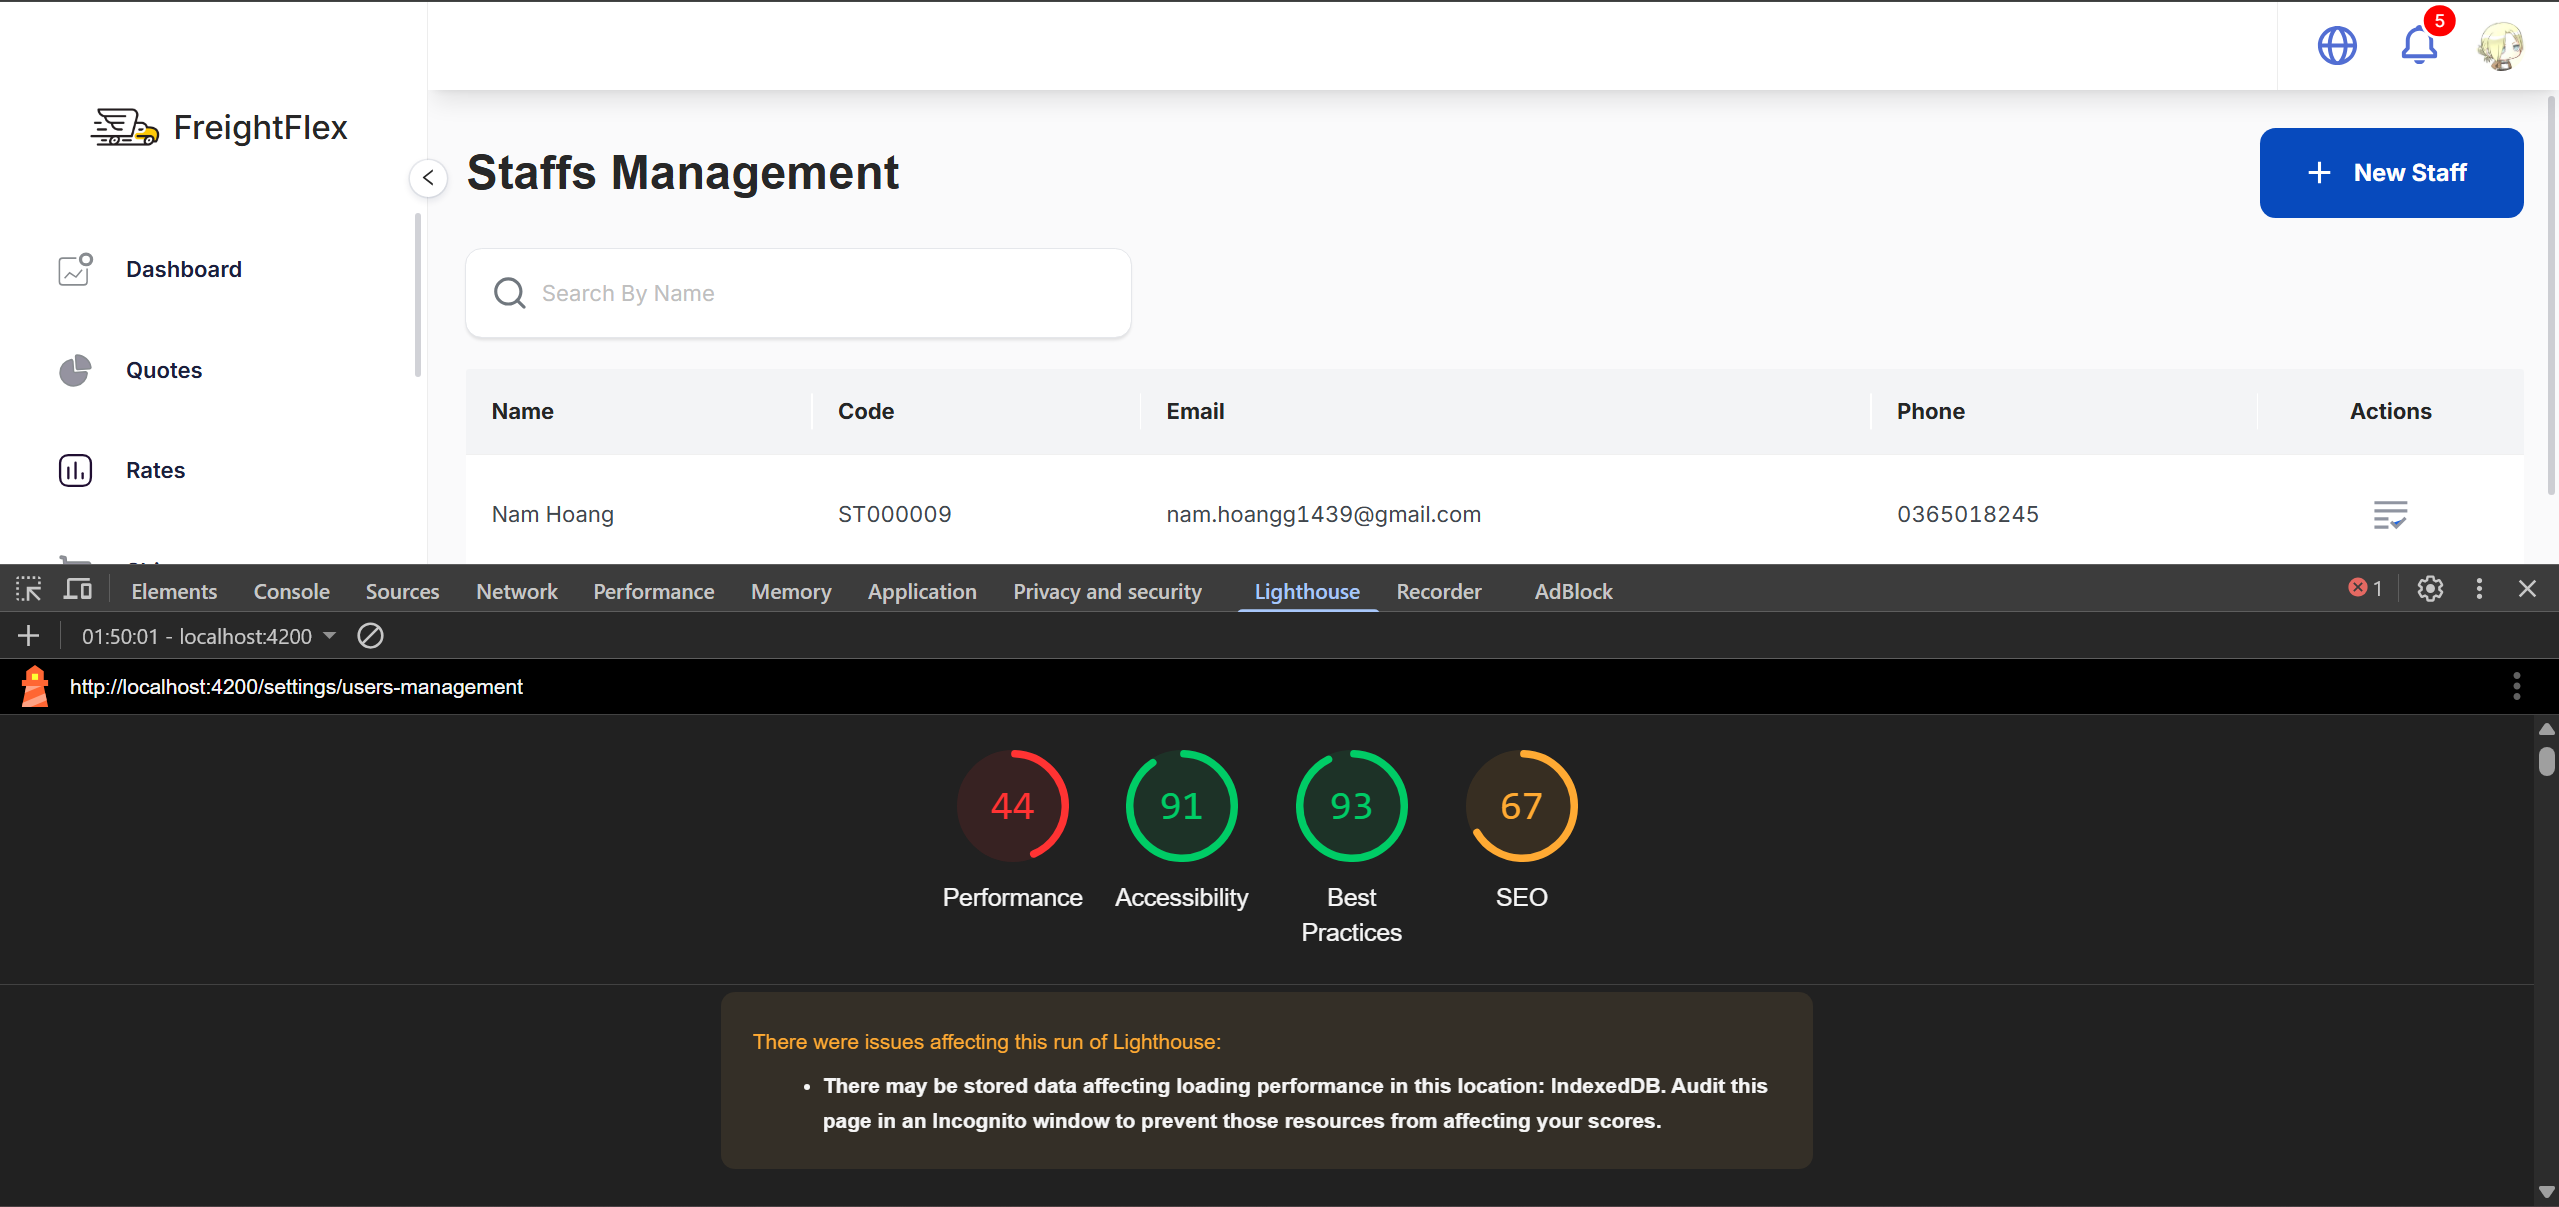
\includegraphics[width=15cm]{graphics/chapter6/staff_before.png}
  \caption{Staff page performance evaluation}
  \label{fig:staff_before}
\end{figure}

\noindent The performance evaluation revealed scores ranging between 40 and 45, which falls below the threshold considered acceptable for modern web applications. In contrast, other metrics achieved values exceeding 60, which is generally regarded as satisfactory performance.

We implemented various optimization strategies based on Lighthouse recommendations, which resulted in notable improvements in the Best Practices metric. However, despite these interventions, the performance score remained consistently low. Analysis indicates this is primarily attributable to the application's dependence on resource-intensive JavaScript libraries and complex computational logic.

Current constraints on time and resources prevent implementation of comprehensive performance optimizations. Nevertheless, a systematic optimization strategy has been developed for implementation in subsequent development phases to address these performance limitations.

